\id{ҒТАМР \href{https://grnti.ru/?p1=65&p2=59&p3=03\#03}{65.59.03}}{}

\begin{articleheader}
\sectionwithauthors{А.К. Суйчинов, Ж.С. Есимбеков, Г.А. Капашева, Г.Е. Жүзжасарова, С.Н. Туменов}{АБАЙ ОБЛЫСЫНДАҒЫ ӘРТҮРЛІ ЖАНУАРЛАР МЕН ҚҰС ЕТІНІҢ ЖӘНЕ СУБӨНІМДЕРІНІҢ ФИЗИКА-ХИМИЯЛЫҚ ҚҰРАМЫН ЗЕРТТЕУ}

{\bfseries
А.К. Суйчинов\alink{https://orcid.org/0000-0003-4862-3293},
Ж.С. Есимбеков\alink{https://orcid.org/0000-0002-8556-9954}\textsuperscript{\envelope },
Г.А. Капашева\alink{https://orcid.org/0009-0001-0735-9783},
Г.Е. Жүзжасарова\alink{https://orcid.org/0009-0003-5470-4345},
С.Н. Туменов\alink{https://orcid.org/0000-0003-3086-1533}
}
\end{articleheader}

\begin{affiliation}
\href{https://rpf.kz/?lang=kk}{Қaзақ қайта өңдеу және тағам өнеркәсіптері ғылыми зерттеу институты} (Семей филиалы), Семей, Қазақстан

\raggedright \textsuperscript{\envelope }Корреспондент-автор: ezhanibek@mail.ru
\end{affiliation}

Бұл мақалада әртүрлі жауарлар мен тауық еті және субөнімдерінің
физика-химиялық көрсеткіштері, рН сутек иондарының концентрациясы,
өнімдердің ылғалды байланыстыру қабілеті және кесу кернеуін зерттеу
көрсеткіштері мен нәтижелері көрсетілген. Тартылған ет өнімдерінен
сынама алынып олардың химиялық құрамын, ылғалды байланыстыру қабілетін,
ортаның белсенді қышқылдылығы (рН) және кесу кернеуін анықтау стандартты
әдістермен жүргізілді. Бұл субөнімдердің химиялық зерттеу нәтижелері
бойынша ақуыздың ең жоғарғы көрсеткішті жылқы жүрегі (20,48 \%),
майлылығы ең төменгі көрсеткішке қойдың бауыры (3,09 \%), күлі ең
жоғарғы сиыр жүрегінде (3,08 \%) болды. Ылғалды байланыстыру қабілетін
зерттеу барысында ең төменгі көрсеткішті тауық бауыры (22,7 \%), ал
ортаның белсенді қышқылдылығын (рН) анықтаған кезде, ең жоғарғы
көрсеткішті сиыр, жылқы, қой қарыныдары (6,6) тең көрсеткішке ие болды.
Сынамаға алынған (рН) нәтижелері бойынша балғын еттің жарамдылығын
көрсетті. Қой еті мен тауық етінің кесу кернеуін анықтау кезіндегі
көрсеткіш нәтижелері бойынша тауық еті (182,0) кПа сынамасы көрсетсе,
қой еті (177) кПа сәйкес төмен екендігі анықталды. Нәтижелер өңдеу
процестерін оңтайландыруда және тұтынушылардың талаптарына сәйкес
келетін өнімдерді әзірлеуде ет өнеркәсібі үшін пайдалы болуы мүмкін.

{\bfseries Түйін сөздер:} жылқы, қой, сиыр және тауық субөнімдері,
физика-химиялық көрсеткіші, ылғалды байланыстыру қабілеті, кесу кернеуі.

\begin{articleheader}
{\bfseries ИЗУЧЕНИЕ ФИЗИКО-ХИМИЧЕСКОГО СОСТАВА РАЗЛИЧНЫХ ЖИВОТНЫХ И ПТИЦЫ,
МЯСА И СУБПРОДУКТОВ В АБАЙСКОМ РАЙОНЕ}

{\bfseries
А.К. Суйчинов,
Ж.С. Есимбеков\textsuperscript{\envelope },
Г.А. Капашева,
Г.Е. Жүзжасарова,
С.Н.Туменов
}
\end{articleheader}

\begin{affiliation}
Казахский научно-исследовательский институт перерабатывающей и пищевой промышленности (Семейский филиал), Семей, Казахстан,

e-mail: ezhanibek@mail.ru
\end{affiliation}

В статье представлены результаты исследования физико-химических
параметров различных видов мяса и субпродуктов. Изучены концентрация
ионов водорода (pH), влагосвязывающая способность, напряжение среза, а
также химический состав продуктов. Для определения химического состава,
влагосвязывающей способности, активной кислотности (pH) среды и
напряжения среза применялись стандартные методы анализа. В результате
исследования установлено, что наибольшее содержание белка
зарегистрировано в сердце конины (20,48\%), а наименьшее содержание жира
--- в бараньей печени (3,09\%). Максимальная зольность отмечена в
говяжьем сердце (3,08\%). Влагосвязывающая способность оказалась
наименьшей у куриной печени (22,7\%). Наибольшие значения активной
кислотности (pH) зафиксированы у говяжьего, конского и бараньего рубца
(6,6). При анализе напряжения среза выявлено, что мясо курицы обладает
более высоким показателем (182,0 кПа), чем мясо баранины (177,0 кПа).
Результаты могут быть полезны для мясной промышленности при оптимизации
процессов переработки и разработки продуктов, соответствующих
требованиям потребителей.

{\bfseries Ключевые слова:} конина, баранина, говяжьи и куриные
субпродукты, физико-химические показатели, влагосвязывающая способность,
напряжение среза.

\begin{articleheader}
{\bfseries STUDYING THE PHYSICAL AND CHEMICAL COMPOSITION OF DIFFERENT
ANIMALS AND POULTRY, MEAT AND BY-PRODUCTS IN THE ABAY DISTRICT}

{\bfseries
A.K. Suichinov,
J.S. Yessimbekov\textsuperscript{\envelope },
G.A. Kapasheva,
G.E. Zhuzzhasarova,
S.N.Tumenov
}
\end{articleheader}

\begin{affiliation}
Kazakh Scientific Research Institute of Processing and Food Industry (Semey branch), Semey, Kazakhstan,

e-mail: ezhanibek@mail.ru
\end{affiliation}

The paper presents the results of the study of physicochemical
parameters of various types of meat and by-products. Hydrogen ion
concentration (pH), water-binding capacity, shear stress, and chemical
composition of the products were studied. Standard analytical methods
were used to determine the chemical composition, water-binding capacity,
active acidity (pH) of the medium and shear stress. The study revealed
that the highest protein content was recorded in horse heart (20.48\%)
and the lowest fat content was recorded in lamb liver (3.09\%). Maximum
ash content was recorded in cattle heart (3.08\%). The water-binding
capacity was lowest in chicken liver (22.7\%). The highest values of
active acidity (pH) were recorded in beef, horse and mutton stomachs
(6.6). ~Analysis of shear stress revealed that chicken meat had a higher
value (182.0 kPa) than lamb meat (177.0 kPa). The results may be useful
for the meat industry in optimizing processing and developing products
that meet consumer requirements.

{\bfseries Key words:} horses, sheep, beef and chicken by-products,
physico-chemical parameters, moisture-binding capacity, shear stress.

\begin{multicols}{2}
{\bfseries Кіріспе.} Қазақстан 2024 жылы бірінші жартыжылдықта шетелге 27,5
мың тоннаға жуық ет экспорттады {[}1{]}. Бұл жаңа қайта өңдеу
кәсіпорындарының іске қосылуы және құс шаруашылығында ет бағытындағы
мемлекеттік қолдаудың кеңеюі осы өнімдер өндірісінің артуына ықпал
етуде. Экспорттың артуына сәйкес әртүрлі жануарлардың субөнімдер
қалдығыда артады. Осы өндірілген субөнімдерді қалдықсыз пайдалану, әрі
өнім өндіру өзекті бағыттардың бірі {[}2{]}. Өңдеу технологияларын
жетілдіру ет шикізатын, әсіресе субөнімдерді өндіру кезек күттірмейтін
өндірістік және әлеуметтік маңызды міндет болып табылады, сондай-ақ
берілген ресурстармен жаңа ұрпақты сапалы азық-түлік өнімдерін өндіруге
жағдай жасау {[}3{]}.

Ет -- бағалы тағамдық өнім. Ағзаның қалыпты жұмыс істеуі үшін қажетті
толық ақуыздардың, майлардың және пайдалы минералды заттардың көзі.
Еттің құрамында 0,6-1,2\% минералды заттар кездеседі және олардың
құрамындағы макроэлементтер (натрий, калий, хлор, магний, кальций және
темір) сонымен қатар микроэлементтерге (йод, мыс, кобальт, марганец,
фтор, қорғасын) жатады. Ет құрамында B1, B2, B6, B9, B12, H, PP, A, D,
E, дәрумендер тобы кездеседі {[}4{]}. Ал субөнімдер (жүрек, бауыр,
қарын) құрамында бұл дәрумендер оданда көп мөлшерде кезедседі {[}5{]}.

Субөнімдер -- ұшаның жеуге жарамды ішкі мүшелері мен сыртқы бөліктері.
Жануарлар салмағының орта есеппен 10-18\% субөнімдері құрайды {[}6{]}.

Ұлт денсаулығы елдің қауіпсіздігін жақсарту үшін шұғыл шараларды қажет
етеді. Дұрыс тамақтану ғана адамның өсуін, қалыпты дамуын және жұмыс
істеуін қамтамасыз ету, аурулардың алдын алуға үлес қосады {[}7{]}.
Жануарлардың еттері (сиыр, жылқы, қой) мен тауық еті және олардың
субөнімдері (жүрек, бауыр, қарын) адамзат рационында маңызды азық болып
табылады. Ет өнімдерінің химиялық құрамының өзгеруі денсаулыққа әсер
етеді, сондықтан бұл көрсеткіштерді зерттеу маңызды.

Бұл жұмыстың мақсаты- жануарлар еттері (сиыр, жылқы, қой) мен тауық еті
және олардың субөнімдері (бауыр, жүрек, асқорту бұлшықеті)
физика-химиялық құрамын, ылғал байланыстыру қабілетін және рН сутек
иондарының концентрациясын, кесу кернеуін зерттеу.

{\bfseries Материалдар мен әдістер.} \emph{Зерттеу объектілері:} Зерттеу
объектісі Абай облысы Семей қаласындағы әртүрлі жануар еті мен тауық
етін сататын арнайы дүкендерінен сатып алынған жылқы, сиыр, қой еттері
мен тауық еті және оның субөнімдері (жүрек, бауыр, қарын, асқорту
бұлшықеті) болды.

\emph{Физика-химиялық зерттеу әдістері}

Жалпы химиялық құрамын сандық анықтау сынаманың бір бөлігінің
әдістерімен жүргізілді. Бұл әдісте бір өнім үлгісіндегі ылғалды, майды,
күлді анықтау үшін жеделдетілген әдіспен ет және сүт өнімдерінің
ылғалдылығы мен майлылығын анықтауға арналған құрылғы қолданылады
{[}8{]}.

\emph{Ортаның белсенді қышқылдылығы (рН)} потенциометриялық әдіспен
рН-метр-150МИ құрылғысы арқылы ерітіндіге екі электродты батыру және рН
мәнін құрылғы шкаласына жазу арқылы анықталды. Ұсақталған өнім сумен
(1:10 қатынасында) ерітінді (судың сүзіндісі) дайындалды. рН 20 °С
температурада 30 минуттан кейін өлшенді {[}9{]}.

\emph{Еттің ылғал байланыстыру қабілетін анықтау.} Ылғалды байланыстыру
қабілеті Р.Грау және Р.Хамм әдісімен анықталды. Бұл әдіс зерттелетін
үлгіні аздап басқан кезде суды шығаруға және оның мөлшерін сүзгі
қағазында қалдырған дақ аймағының өлшеміне қарай анықтауға бағытталған
{[}10{]}.

\emph{Кесу кернеуін анықтау}

Зерттеу үлгілері арнайы құрылғыда сынамаларды кесу арқылы жүзеге асады.
Айналмалы құбырлы пышаққа өнімнің бір бөлігін аздап басу арқылы
сынамалар арнайы құрылғыда кесілді. Алынған диаметрі 0,01 м болатын
тегіс цилиндрлік үлгі итергіш көмегімен жүзеге асты. Сынамаларды кесуге
арналған арнайы құрылғы болмаған жағдайда, сынаманы қабырғалары 0,02Х
0,02 м шаршы түрінде қолмен кесіп алды.

Дайын өнім сынамасы үстелге мұқият орналастырылды. Сынаманы кесуге
қажетті күш құрылым дисплейінде жазылды. Содан кейін құрылғының жұмыс
режимі жоғарыда сипатталғандай орнатылды. «Бастау» түймесін басу арқылы
үлгіні кесетін кесу құралы қозғалысқа келтірілді. Өлшеу кезінде параметр
мәндері экранда пайда болды және құрылғының жадында автоматты түрде
жазылды. Осыдан кейін барлық өлшеу деректері компьютерде өңделеді. Бұл
жағдайда кесу кернеуінің мөлшері өнімге әсер ететін күшті формула (1)
бойынша өнімнің бетінен өтетін жолдың ауданына бөлу арқылы анықталды:

\begin{equation}
\theta_{\text{ср}}=\frac{P}{F},\text{ Па}
\end{equation}

Р-кесу күші, Н;

F-кесу бетінің ауданы, м\textsuperscript{2}:
$F=\pi R^{2}$;

R-үлгінің радиусы, м.

\emph{Статистикалық талдау}

Өлшеу нәтижелерін өңдеу Excel-2016 бағдарламасының көмегімен жүзеге
асырылды. Талдау нәтижелері р≤0,05 кезінде статистикалық маңызды болды.
Деректер орташа ± стандартты ауытқу ретінде ұсынылған. Үлгілер
арасындағы айырмашылықтардың маңыздылығын бағалау үшін бір жақты
дисперсия талдауы (ANOVA) жүргізілді.
\end{multicols}

\begin{table}[H]
\caption*{1 - кесте. Еттің химиялық құрамы}
\centering
\begin{tblr}{
  width = \linewidth,
  colspec = {Q[208]Q[231]Q[171]Q[171]Q[154]},
  cells = {c},
  hlines,
  vlines,
}
\textbf{Ет түрі} & \textbf{Ылғалдылығы} & \textbf{Ақуызы} & \textbf{Майы} & \textbf{Күлі} \\
Сиыр             & 70.40±1,25           & 18.88±0,37      & 9.68±0,17*    & 0.97±0,01     \\
Қой              & 67.98±0,76           & 18.60±0,31      & 11.86±0,16*   & 0.97±0,01     \\
Жылқы            & 71.21±1,17*          & 20.63±0,29*     & 6.44±0,14*    & 1.13±0,01*    \\
Құс еті (тауық)  & 66.49±0,85           & 18.51±0,23      & 13.21±0,20*   & 0.99±0,02     
\end{tblr}
\caption*{\normalfont\emph{* бағандардағы мәндер айтарлықтай ерекшеленеді (p<0.05)}}
\end{table}

\begin{multicols}{2}
{\bfseries Зерттеу нәтижелері.} Зерттеу барысында жылқы, сиыр, қой еттері
мен тауық еті және олардың субөнімдерінің (бауыр, жүрек, қарын, асқазан
бұлшықеті) физика-химиялық құрамы, рН сутек иондарының концентрациясы,
ылғал байланыстыру қабілеті және кесу кернеуі анықталып кестелерде,
диаграммаларда көрсетілді.

\emph{Химиялық құрамын зерттеу}

Зерттеуге сынама ретінде сиыр, жылқы, қой және тауық еттері мен олардың
субөнімдері (бауыр, жүрек, қарын, асқазан бұлшықеті) алынды. Олардың
физика-химиялық құрамы анықталды. Еттің химиялық құрамы 1- кестеде
көрсетілген.

Талданатын ет түрлерінің ішінде жылқы етінде ылғалдың ең көп мөлшері
-71,21\%, одан кейін сиыр еті-70,40\% байқалды. Сәйкесінше қой мен
тауықтың ылғалдылығы 67,98\% және 66,49\% төмен болды. Жылқы еті мен
сиыр етіндегі ылғалдың жоғары мөлшері бұлшықет талшықтарының құрамына
{[}11{]} және ылғалдылық деңгейіне кері пропорционал болатын бұлшықет
ішілік майдың аз болуына байланысты болуы.

Ақуыз еттің биологиялық және функционалдық қасиеттерін анықтайтын ең
маңызды тағамдық құрамы болып табылады. Ең жоғары ақуыз мөлшері жылқы
етінде 20,63\%, сиыр етінен (18,88\%), қой етінен (18,60\%) және тауық
етінен (18,51\%) асып түсті. Жылқы еті құнды ақуыздар құрамы бойынша
сиыр, қой және тауық етінен кем болмайтыны анықталған. Оның құрамында
барлық алмастырылмайтын аминышқылдар бар және олар өте қолайлы қатынаста
орналасқан {[}12{]}.

Майдың мөлшері дәміне, құрамына және калориясына әсер етеді. Тауық еті
майдың ең жоғары мөлшерін - 13,21 \%, одан кейін қой еті - 11,86\%, сиыр
еті - 9,68\% және жылқы еті - 6,44\% көрсетті. Тауықтың аяқы мен
жамбасындағы майдың көп мөлшері құстың анатомиясына сәйкес келеді, онда
бұл бөліктерге көп май жиналады. Қой етіндегі майдың салыстырмалы түрде
жоғары мөлшері май тінінің таралуының түрлік ерекшеліктерімен байланысты
болуы мүмкін. Жылқы етіндегі майдың аздығы оның денсалуығын ойлайтын
тұтынушыларды тарта алатын майсыз ет ретінде жіктелуін көрсетеді
{[}13{]}.

Күл әртүрлі физиологиялық функцияларды орындау үшін қажет және ет
құрамындағы минералдардың жалпы мөлшері. Жылқы етінде күл мөлшері ең
жоғары - 1,13\% болды, бұл сиыр етімен (0,97\%), қой етімен (0,97\%)
және тауықпен (0,99\%) салыстырғанда минералды құрамның жоғары екендігін
көрсетеді. Жылқы етіндегі күлдің жоғарылауы жануарлар түрлерінің
рационына, зат алмасуындағы немесе бұлшықет құрамының айырмашылығына
байланысты болуы мүмкін.

Осылайша, салыстырмалы дәлелдер жылқы етінің ылғалдылығы мен ақуызы ең
жоғары және майы ең төмен екенін көрсетеді. Керісінше, тауық етінде,
әсіресе аяқтар мен жамбастарда, зерттелген барлық ет түрлерінің ішіндегі
ең жоғары май және ең аз ылғал мен ақуыз бар. Май мен ылғалдылық
арасындағы кері байланыс барлық үлгілерде байқалады. Тауық еті мен қой
еті сияқты майы жоғары еттердің ылғалдылығы төмен болды. Бұл құбылысты
бұлшықет тініндегі судың маймен алмастырылуымен түсіндіруге болады,
өйткені май мөлшері артады {[}14{]}.

Әртүрлі жануарлар мен тауықтың субөнімдерінің химиялық құрамын талдау
кезінде олардың мүшелері арасындағы айырмашылықтарды анықтады.
(p\textless0,05). Сиыр еті, қой еті, жылқы еті мен тауық еті және
субөнімдерін талдау кезінде ылғал, ақуыз, май және күл құрамындағы
айырмашылықтар табылды.

\emph{Жүректің химиялық көрсеткіші}

Ылғалдылық құрамы: Жүректің ылғалдылығы жануарлар түрлері арасында
айтарлықтай өзгерді (p \textless0,05). Қой жүрегінде ең жоғары
ылғалдылық 80,9\% болса, бұл құс жүрегінен (76,3\%), сиыр етінен
(74,53\%) және жылқы жүрегінен (74,46\%) жоғары көрсеткіш көрсетті.
Қойдың жүрегіндегі ылғалдың жоғарылауы жүрек тінінде судың сақталуына
әсер ететін түрге тән метаболикалық сипаттамаларға байланысты болуы
мүмкін. Субөнімдердің химиялық құрамы 2 -- кестеде көрсетілген.

Ақуыздың құрамы: жылқы жүрегі ақуыздың ең жоғары деңгейіне - 20,48\% ие
болды, сиыр жүрегінен (18,52\%), құс жүрегінен (15,42\%) және қозы
жүрегінен (14,12\%) (p \textless{} 0,05) айтарлықтай асып түсті. Жылқы
жүрегіндегі ақуыздың жоғары деңгейі бұлшықеттердің тығыздығын және май
мен ақуыздың арақатынасының төмендігін көрсетеді, бұл оны майсыз
ақуыздың құнды көзі етеді.

Май құрамы: құстың жүрегінде майдың ең көп мөлшері бар - 6,68\%, бұл
жылқы жүрегінен (5,31\%), сиыр жүрегінен (3,87\%) және қой жүрегінен
(3,48\%) (p \textless{} 0,05) айтарлықтай көп. Құстың жүрегіндегі майдың
көп мөлшері липидтер алмасуының және майдың жиналуының түрлік
ерекшеліктеріне байланысты болуы мүмкін.
\end{multicols}

\tcap{2 - кесте. Субөнімдердің химиялық құрамы, \%}
\begin{longtblr}[
  label = none,
  entry = none,
]{
  width = \linewidth,
  colspec = {Q[258]Q[221]Q[163]Q[146]Q[146]},
  cells = {c},
  cell{2}{1} = {c=5}{0.934\linewidth},
  cell{6}{1} = {c=5}{0.934\linewidth},
  cell{10}{1} = {c=5}{0.934\linewidth},
  cell{14}{1} = {c=5}{0.934\linewidth},
  hlines,
  vlines,
}
\textbf{Ет түрі}        & \textbf{Ылғалдылығы} & \textbf{Ақуызы} & \textbf{Майы} & \textbf{Күлі} \\
\textit{\textbf{Сиыр}}  &                      &                 &               &               \\
Жүрек                   & 74.53±1,31           & 18.52±0,25      & 3.87±0,04     & 3.08±0,05     \\
Бауыр                   & 75.81±1,22           & 18.96±0,19      & 3.78±0,04     & 1.45±0,02*    \\
Қарын                   & 77.12±0,88           & 15.73±0,25*     & 5.85±0,07*    & 1.3±0,02*     \\
Қой                     &                      &                 &               &               \\
Жүрек                   & 80.90±1,13           & 14.12±0,19*     & 3.48±0,06*    & 1.50±0,02     \\
Бауыр                   & 75.57±1,02*          & 19.85±0,41*     & 3.09±0,04*    & 1.49±0,02     \\
Қарын                   & 83.45±0,87           & 11.60±0,13*     & 4.04±0,06*    & 0.91±0,01*    \\
Жылқы                   &                      &                 &               &               \\
Жүрек                   & 71.46±1,04           & 20.48±0,43*     & 5.31±0,09*    & 2.75±0,03*    \\
Бауыр                   & 75.25±0,60           & 19.40±0,22*     & 3.89±0,05*    & 1.46±0,02     \\
Қарын                   & 75.87±1,24           & 16,00±0,23*     & 6.40±0,07*    & 1.73±0,03     \\
\textit{\textbf{Тауық}} &                      &                 &               &               \\
Жүрек                   & 76.30±1,15           & 15.42±0,25*     & 6.68±0,10*    & 1.60±0,02     \\
Бауыр                   & 74.37±1,29           & 18.91±0,20      & 5.29±0,06*    & 1.43±0,02     \\
Асқазан бұлшықеті       & 74.30±0,88           & 19.49±0,33      & 4.94±0,08*    & 1.28±0,02*    
\end{longtblr}
\vspace{-2.5em}
\begin{center}
\emph{* бағандардағы мәндер айтарлықтай ерекшеленеді (p\textless0.05)}
\end{center}

\begin{multicols}{2}
Күл құрамы: сиыр жүрегінде күл мөлшері ең жоғары болды - 3,08\%, бұл
жылқы жүрегінен (2,75\%), құс жүрегінен (1,6\%) және қой жүрегінен
(1,5\%) (p \textless{} 0,05) айтарлықтай жоғары болды. Бұл сиыр етінің
жүрегінде минералдар көп болуын көрсетеді, бұл оның тағамдық құндылығын
арттырады {[}15{]}.

\emph{Бауырдың химиялық құрамы}

Ылғалдылық: бауыр үлгілеріндегі ылғалдылық аздап өзгерді. Сиыр бауырында
75,81\% ылғал болса, одан кейін қой бауыры (75,57\%) және жылқы бауыры
(75,25\%) көрсетті. Құстың бауыры ылғалдың аздығымен
ерекшеленді-74,37\%. Бұл айырмашылықтар статистикалық маңызды емес (p
\textgreater{} 0,05), бұл жануарлардың осы түрлерінің бауырындағы
ылғалдылық салыстырмалы түрде бірдей екенін көрсетеді.

Ақуыздың мөлшері: қой етінің бауыры ақуыздың ең жоғары мөлшерін көрсетті
- 19,85\%, бұл жылқы бауырынан (19,4\%), сиыр бауырынан (18,96\%) және
құс бауырынан (18,91\%) сәл жоғары. Айырмашылықтар статистикалық маңызды
емес (p \textgreater{} 0,05), бұл осы түрлердің бауырындағы ақуыздың
ұқсас құрамын көрсетеді.

Май құрамы: майдың мөлшері әр түрлі болды, құстың бауырында майдың ең
көп мөлшері 5,29\% болды, бұл қой бауырынан (3,09\%), сиыр бауырынан
(3,78\%) және жылқы бауырынан (3,89\%) (p \textless{} 0,05) едәуір көп.
Құс бауырындағы майдың жоғарылауы құс бауырында липидтердің жиналуының
жоғарылауымен байланысты болуы мүмкін.

Күл құрамы: бауырдағы күл мөлшері салыстырмалы түрде бірдей және тауық
бауырында 1,43\%-дан қой бауырында 1,49\%-ға дейін кездесті. Бұл шамалы
айырмашылықтар статистикалық маңызды емес (p \textgreater{} 0,05), бұл
әртүрлі бауыр тіндеріндегі салыстырмалы минералды құрамды көрсетеді.

\emph{Қарын мен асқазан бұлшықетінің химиялық құрамы}

Ылғалдылық: қой етінің қарыны ең жоғары ылғалдылыққа ие болды-83,45\%,
сиыр қарыны (77,12\%), жылқы қарыны (75,87\%) және тауықтың асқазан
бұлшықеті (74,3\%) (p \textless{} 0,05). Қойдың қарынындағы ылғалдың
жоғары болуы ас қорыту физиологиясындағы айырмашылықтарды және қарынның
ашыту процестеріндегі рөлін көрсетуі мүмкін, бұл судың көп сақталуына
әкеледі.

Ақуыздың мөлшері: құс асқазанында ақуыздың ең жоғары мөлшері 19,49\%
анықталса, бұл жылқы етінен (16,0\%), сиыр етінен (15,73\%) және қой
етінен (11,6\%) айтарлықтай жоғары (p \textless0,05) екендігін
көрсетеді. Бұл күйіс қайыратын малдың қарындарымен салыстырғандағы
құрылымдық және функционалдық ерекшеліктерге байланысты тауық асқазан
бұлшықетінің ақуызға бай екендігін көрсетеді {[}16{]}.

Майдың мөлшері: майдың ең жоғары мөлшері жылқының қарынында 6,4\% болса,
бұл сиыр етінен (5,85\%), құс етінен (4,94\%) және қой етінен (4,04\%)
айтарлықтай (p \textless0,05) жоғары болды. Жылқының қарнындағы майдың
жоғарылауы диеталық факторларға және жылқыларға ғана тән майдың
жиналуына байланысты болуы мүмкін.

Күлдің мөлшері: күлдің ең жоғары мөлшері жылқы қарынында 1,73\% болса,
бұл сиыр етінен (1,3\%), құс етінен (1,28\%) және қой етінен (0,91\%),
(p \textless0,05) жоғары болды. Бұл жылқының қарнындағы минералды
құрамның жоғары екенін көрсетеді, бұл қоректік тұрғыдан пайдалы болуы
мүмкін {[}17{]}.

\emph{Ортаның белсенді қышқылдылығы (рН) мен ылғалды байланыстыру
қабілетін анықтау}

Зерттеудің келесі кезеңінде әртүрлі жануарлардың -- сиыр, қой, жылқы
және тауық етінің рН және ылғал байланыстыру қабілеті (ЫБҚ) зерттелді
(1-сурет). Бұл нәтижелер әртүрлі ет түрлерінің арасындағы рН және ЫБҚ
мәніндегі айырмашылықтарды көрсетеді.

Бұл зерттеуде жылқы етінде ең төменгі рН 5,9 болды, бұл басқа еттермен
салыстырғанда ет ақуыздарының изоэлектрлік нүктесіне жақынырақ. Осыған
қарамастан жылқы еті салыстырмалы түрде жоғары ЫБҚ 72,4\% көрсетті, бұл
сиыр етінен сәл ғана төмен болды, ең жоғары ЫБҚ 73,6\% және рН 6,1 болды
{[}18{]}. Бұл ақуыз сияқты рН-дан басқа факторлардың ЫБҚ-ге әсер етуде
маңызды рөл атқаратынын көрсетеді. Зерттелетін ет түрлерінің ішінде ең
жоғары ақуыз мөлшері жылқы етінде -- 20,63\%, ал майлылығы -- 6,44\%
болды. Ақуыздың жоғары мөлшері ылғалмен байланысу қабілетінің
жоғарылауына ықпал етеді, өйткені ақуыздарда су молекулаларымен
әрекеттесетін көптеген гидрофильді аймақтар бар, осылайша бұлшықет
құрылымында көбірек су сақталады. Сонымен қатар, майдың төмен мөлшері
ЫБҚ жоғарылауына ықпал етуі мүмкін, өйткені май суды ұстап тұру үшін
пайдаланылуы мүмкін кеңістікті алады {[}19{]}.

Сиыр еті рН 6,1 және ақуыз мөлшері 18,88\% ең жоғары деңгейін ЫБҚ 73,6\%
көрсетті. Салыстырмалы түрде жоғары рН ақуыздардағы теріс заряды
арттыруға көмектеседі, олардың электростатикалық итеру арқылы суды ұстау
қабілетін арттырады. Ақуыздың қалыпты мөлшері ақуыздың сумен әрекеттесуі
нәтижесінде судың байланысуына ықпал етеді.

Қой мен құс етінің рН мәндері 6,3 жоғары болды. Дегенмен, ЫБҚ
көрсеткіштері сиыр және жылқы етінен қой еті 67,3\% және құс еті 63,6\%
төмен болды. Бұл айырмашылық ақуыз мөлшерінің төмен болуына байланысты
болуы мүмкін - қой еті үшін 18,60\% және құс еті үшін 18,51\% - және
майдың жоғарылығы - қой еті үшін 11,86\% және құс еті үшін 13,21\%.
Майдың жоғары мөлшері суды байланыстыру қабілетін төмендетуі мүмкін,
өйткені май суды байланыстырмайды және ақуыздар мен су молекулалары
арасындағы өзара әрекеттесуге физикалық кедергі келтіруі мүмкін.
Ақуыздың төмен мөлшері суды байланыстыратын гидрофильді орындардың аз
болуын білдіреді, бұл жалпы ЫБҚ азайтады {[}20{]}.
\end{multicols}

\begin{figure}[H]
	\centering
	\begin{subfigure}{0.48\textwidth}
		\centering
		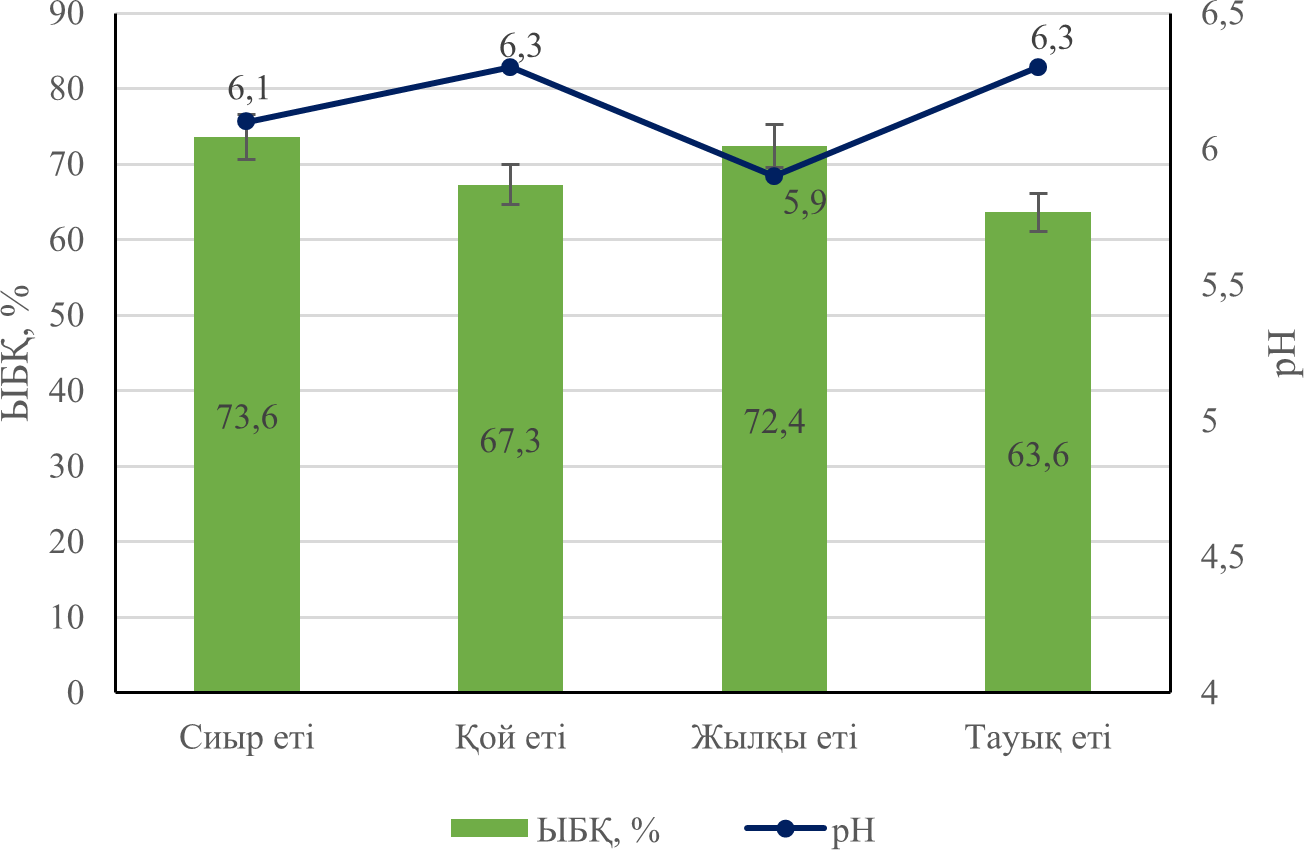
\includegraphics[width=\textwidth]{media/pish4/image1}
		\caption*{1 - сурет. Әртүрлі еттің ылғал байланыстыру қабілеті және pH мәні}
	\end{subfigure}
	\begin{subfigure}{0.48\textwidth}
		\centering
		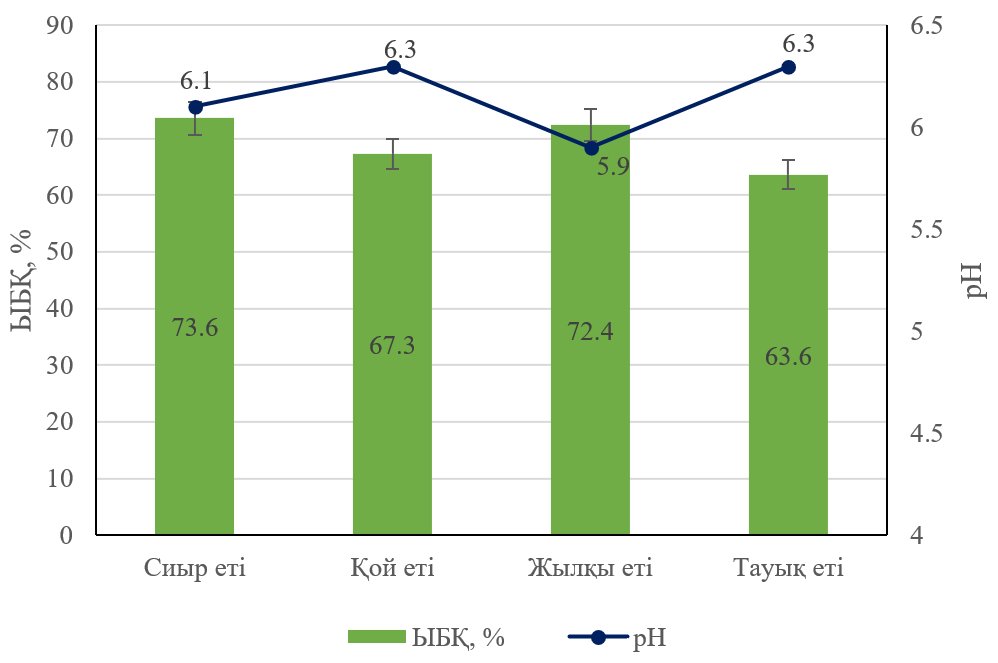
\includegraphics[width=\textwidth]{media/pish/image5}
		\caption*{2 - сурет. Cиыр субөнімдерінің (жүрек, бауыр, қарын) ылғал байланыстыру қабілеті және pH мәні}
	\end{subfigure}
\end{figure}

\begin{multicols}{2}
Жалпы, еттің суды байланыстыру қабілетіне факторлардың жиынтығы әсер
етеді, соның ішінде рН, ақуыз мөлшері, май мөлшері және бұлшықет
талшықтарының сипаттамалары. Ал рН суды байланыстыру қабілетінде маңызды
рөл атқарса да, ақуыз мөлшері еттің жалпы суды ұстау қабілетіне
айтарлықтай үлес қосады. Жоғары ақуыз мөлшері, жылқы етінде
байқалғандай, рН изоэлектрлік нүктеге жақын болса да, ЫБҚ жоғарылайды.
Керісінше, майдың жоғарылауы бұлшықет құрылымындағы суды байланыстыратын
ақуыздар үшін бос орынды азайту арқылы ЫБҚ-ке теріс әсер етуі мүмкін.
\end{multicols}

\begin{figure}[H]
	\centering
	\begin{subfigure}{0.48\textwidth}
		\centering
		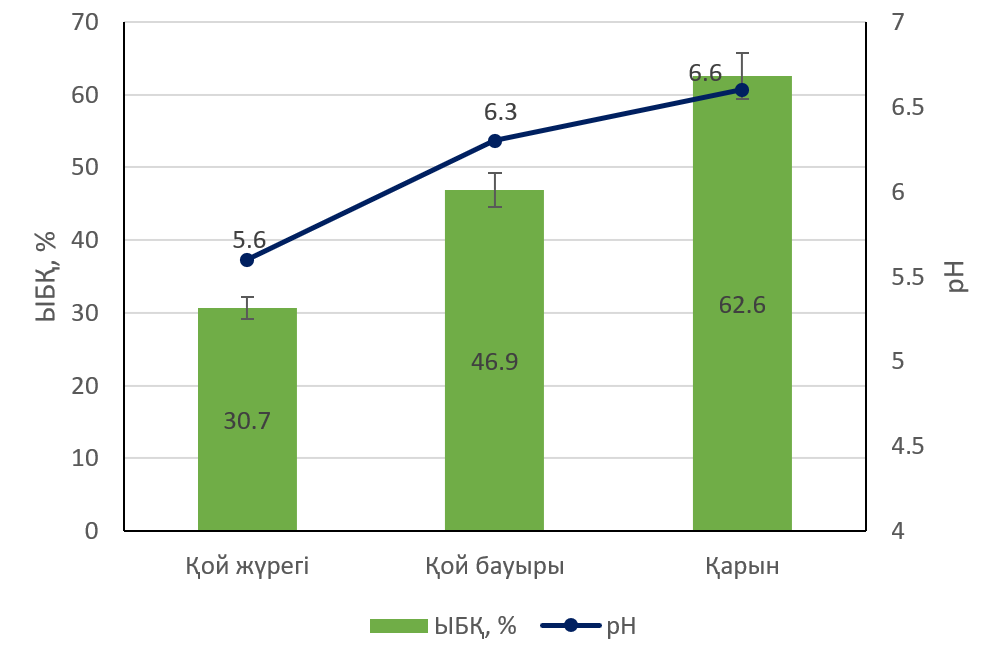
\includegraphics[width=\textwidth]{media/pish/image6}
		\caption*{3 - сурет. Қой субөнімдерінің (жүрек, бауыр, қарын) ылғал байланыстыру қабілеті және pH мәні}
	\end{subfigure}
	\begin{subfigure}{0.48\textwidth}
		\centering
		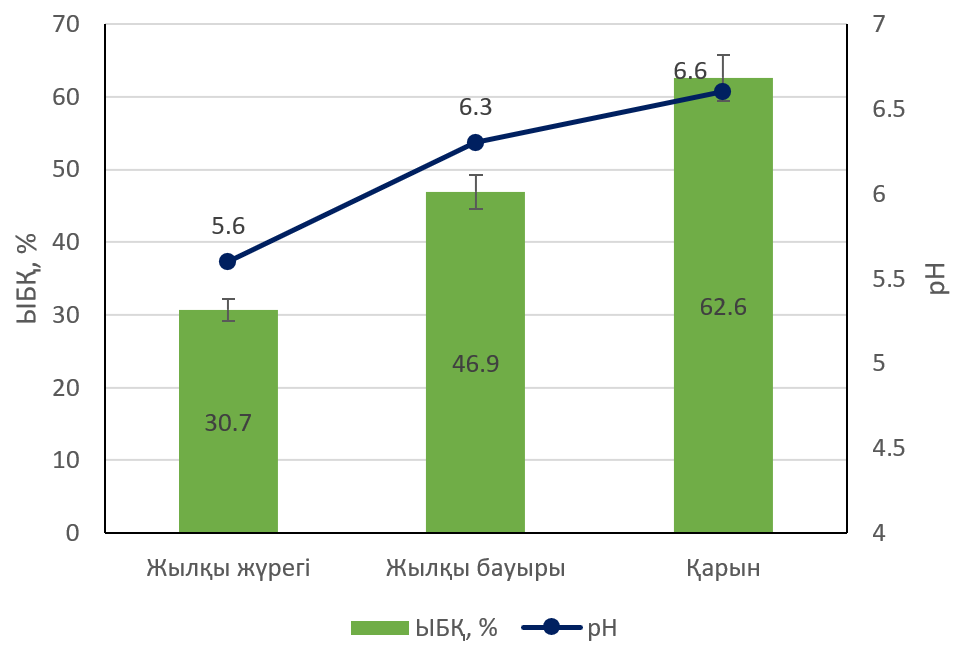
\includegraphics[width=\textwidth]{media/pish/image7}
		\caption*{4 - сурет. Жылқы субөнімдерінің (жүрек, бауыр, қарын) ылғал байланыстыру қабілеті және pH мәні}
	\end{subfigure}
\end{figure}

\begin{multicols}{2}
Әртүрлі жануарлардың субөнімдерінің ылғалды байланыстыру қабілетін
салыстырмалы түрде қарасақ жылқы мен қой жүрегі ЫБҚ 30,7\% тең көрсетті.
Ал сиыр жүрегі 29,1\% төмен көрсеткішке ие болды (2-сурет). Жылқы мен
қой бауыры сәйкес 46,9 \% тең, сиыр жүрегі 45.6\% аз. Жылқы мен қой
қарыны 62,6\% тең, ал сиыр қарыны 29,6 \% төмен көрсеткіш көрсетті
(3-4-сурет). Сиыр жүрегі ең жоғары рН-6,29 ал барлық жануарлар бауырында
рН-6,3 және қарыны рН-6,6 тең болды.
\end{multicols}

\begin{figure}[H]
	\centering
	\begin{subfigure}{0.48\textwidth}
		\centering
		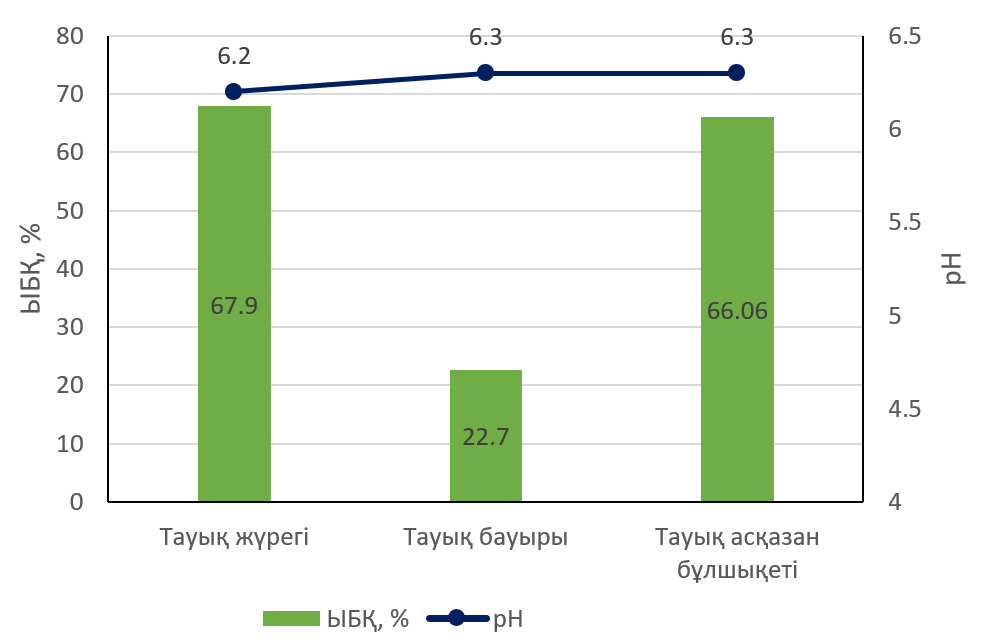
\includegraphics[width=\textwidth]{media/pish/image8}
		\caption*{5 - сурет. Тауық субөнімдерінің (жүрек, бауыр, асқазан бұлшықеті) ылғал байланыстыру қабілеті және pH мәні}
	\end{subfigure}
	\begin{subfigure}{0.48\textwidth}
		\centering
		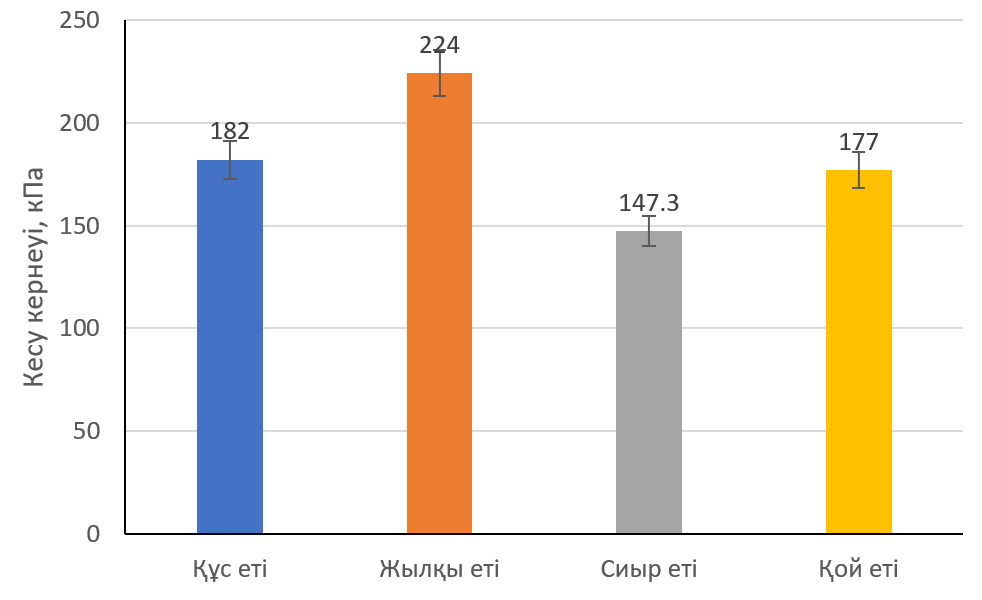
\includegraphics[width=\textwidth]{media/pish/image9}
		\caption*{6-сурет. Әртүрлі еттің кесу кернеуі}
	\end{subfigure}
\end{figure}

\begin{multicols}{2}
Тауық субөнімдерінің ЫБҚ тоқталатын болсақ, ең жоғарғы көрсеткішті
жүрегі 67,9 \%, ал ең төмен көрсеткішті бауыры 22,7\% байқауға болады.
Тауық жүрегі ең төменгі рН -- 6,2 көрсетсе, сәйкесінше бауыры мен
асқазан бұлшықеті рН -- 6,3 тең келді (5-сурет).

\emph{Кесу кернеуі.} Әртүрлі жануарлар мен құс етінің кесу кернеуінің ең
жоғары мәні жылқы етінде 224 кПа байқалса, ең төменгі мәнді 147,3 кПа
сиыр етінде анықталды. Бұл айырмашылық ең алдымен әртүрлі жануарлар мен
құс етінің құрамы және құрылымымен түсіндіріледі. Сонымен қатар жылқы
етінің дәнекер тіндері басым, бұл қаттылық пен серпімділік береді. (6 --
сурет).

Етті кесу кернеуі май мен ылғалға байланысты текстуралық сипаттамаларға
байланысты. Бұл параметрлер ет жұмсақтығы мен қаттылығы сияқты
механикалық қасиеттеріне әсер етеді. Ылғалдылықтың жоғары мөлшері етті
жұмсақ етеді, өйткені су бұлшықет талшықтарын жұмсартады. Ылғал азайған
сайын ет тығызырақ және қаттырақ болады, бұл кесу кернеуін арттырады.
Бұл әсіресе ылғалдың бір бөлігі жоғалған кезде термиялық өңдеу
процесінде байқалады. Май бұлшықет талшықтары арасында "майлау" қызметін
атқарады, бұл олардың кесілген кездегі үйкелісін азайтады. Бұл етті
жұмсақ етеді және кесу кернеуін азайтады. Майы аз ет, әдетте, жұмсартқыш
әсерінің аздығына байланысты кесу кернеуі жоғары болады. Май, ылғал және
кесілген кернеу арасындағы байланыс. Май мен ылғалдың үйлесімі еттің
органолептикалық қасиеттерін жақсарта отырып, кесу кернеуін төмендетеді
{[}21{]}.

{\bfseries Нәтижелер мен талқылау.} Сиыр еті - әлемде көптеген елдерінің
тағамдарында кеңінен қолданылатын танымал ет өнімі. Бұл жоғары сапалы
ақуыз мен қоректік заттардың көзі {[}22{]}. Жылқы мен тауық еттері төмен
калориялы, ақуызға бай, денсаулыққа пайдалы тағамдар қатарына жатады.
Олар диеталық мәзірлерде жиі қолданылады және салауатты өмір салтын
ұстанатын адамдар үшін ұсынылады {[}23{]}. Қой етінің кұрамындағы ақуыз
сиыр етінікімен бірдей, ал майы жоғары қуатты. Сиыр етінікімен
салыстырғанда қой етіндегі холестерин мөлшері 2-2,5 есе аз, ал маңызды
калыций, фосфор, мыс, мырыш секілді минералды элементтері, керісінше көп
{[}24{]}.

Субөнімдері --ең маңызды аминқышқылдарының, витаминдер мен минералдардың
көзі және көбінесе жоғары сапалы ақуызға бай болып табылады. Сиыр жүрегі
-- субөнімдердің ең маңызды түрлерінің бірі оның жүрегінде ең көп
пайдалы мөлшерде В12 дәрумені және қоректік заттар темір, барлық тоғыз
маңызды алмастырылмайтын амин қышқылы кездеседі {[}25{]}. Сиыр қарын
құрамында жалпы ақуыз 17,1 г, коллаген 10,5 г құрайды. Аминқышқылдарының
құрамы бойынша қарын маңызды алмастырылмайтын аминқышқылдарының толық
жиынтығын қамтиды {[}26{]}. Жылқы және қойдың бауыры, жүрегі, және
қарынының тағамдық диеталық қасиеттері ерекше, олар адам ағзасына
пайдалы болып саналады. Жылқы бауырында темірдің жоғары мөлшері
қаназдықтың алдын алады, гемоглобинді көтеруге көмектеседі. А дәрумені
көздің көру қабілетін жақсартады, иммундық жүйені нығайтады. Қой жүрек
құрамында калий мен магний жүрек-қан тамырлары жүйесінің жұмысын
жақсартады. Жылқы қарын негізінен ақуыздан және аз мөлшердегі майдан
тұрады және құрамында коллаген мен басқа да пайдалы заттар бар. Ал
тауықтың субөнімдері (жүрегі, бауыры, асқазан бұлшықеті) дәрумендерге,
минералдарға және ақуызға бай, ал олардың энергетикалық құндылығы жоғары
емес, бұл оларды диеталық тағам ретінде де пайдалануға мүмкіндік береді.

Жүргізілген зерттеу нәтижесінде әртүрлі жануарлар мен құс етінің
химиялық кұрамы бойынша ең жоғарғы ылғылдылықты жылқы етінде 77,21\%, ең
төменгі ылғалдылықты құс еті 66,49 \% ие болды. Ақуызына тоқталатын
болсақ, ең жоғарғы көрсеткіш жылқы еті 20,63 \% байқалса, төмен
көрсеткішті 18,51 \% құс етінде байқалды. Майлылығы бойынша жоғарғы
көрсеткішті құс еті 13,21\%, ең төменгі жылқы етінде 6,44 \% анықталды.
Күлі ең жоғарғысы жылқы етінде 1,13 \% байқалды. Осы аталған өнімдердің
субөнімдерінің химиялық көрсеткіші нәтижесінде ең жоғарғы ылғалдылықты
қой қарыны 83,45 \%, ақуызы ең төмен қой қарыны 11,60 \%, ал майлылығы
ең жоғары 6,40\% жылқы қарынында, күлі төмен мәнге қой қарынында 0,91 \%
көрсетті. ЫБҚ зерттеу нәтижесі бойынша ең жоғарғы ЫБҚ сиыр еті 73,6 \%
көрсетсе, ал ең төменгі орта белсенді қышқылдылық көрсеткішті жылқы еті
рН=5,9 екендігі байқалды.

{\bfseries Қорытынды.} Зерттеу нәтижелері ет өнімдерін өндірудің
технологиялық процестерінде әртүрлі жануарлар мен құс еті және оның
субөнімдерін қолданудың орындылығын негіздейді. Жылқы етінің ақуыз
құрамының жоғары нәтиже көрсетуі оның майсыз табиғаты мен ақуыздық
фракцияны шоғырландыратын майдың аздығына байланысты болуы мүмкін.
Сәйкесінше сиыр, қой және тауық етіндегі ұқсас ақуыз мөлшері осы еттегі
бұлшықет ақуыздың салыстырмалы кескінін көрсетеді. Тауықтың аяғы мен
жамбасындағы майдың көп мөлшері құстың анатомиясына сәйкес келеді, онда
бұл бөліктер белсенді және көп май жинайды. Қой етіндегі майдың
салыстырмалы түрде жоғары мөлшері май тінінің таралуының түрлік
ерекшеліктерімен байланысты болуы мүмкін. Жылқы етіндегі майдың аздығы
оның денсаулығын ойлайтын тұтынушыларды тарта алатын майсыз ет ретінде
жіктелуін көрсетеді.

Әртүрлі жануарлардан алынған субөнімдерде ылғалдың, ақуыздың, майдың
және күлдің құрамындағы айтарлықтай айырмашылықтар байқалды. Бұл
деректер рационда жанама өнімдерді пайдалану кезінде жануарлар түрлерін
таңдаудың маңыздылығын көрсетеді. Субөнімдер қоректік заттардың алуан
түрін қамтамасыз етеді және оларды диетаға қосу тағамдық артықшылықтарға
және жануарлар ресурстарын тұрақты пайдалануға ықпал етеді. Оларды
пайдалану тағамды жоғары сапалы ақуызбен және маңызды аминқышқылдарымен
байытуға ықпал етеді, бұл дұрыс тамақтану мен заман талабына сәйкес
ұтымды пайдаланудың тенденцияларына сәйкес келеді. Жүргізілген
зерттеулердің нәтижелері әртүрлі жануарлар мен құс еті және оның
субөнімдері бойынша норма талаптарына сай екендігін көруге болады.
Сондықтан мұндай зерттеулер ет және субөнімдерін одан әрі өңдеу және
дамыту үшін пайдалы болады.

Өндірушілер үшін диеталық тағам өндіру мақсатында тауық, жылқы еттерін
ұсынуға болады. Себебі олардың химиялық құрамы мен биологиялық құндылығы
бойынша, оның ішінде жоғары ақуыз, төмен майлылық және маңызды
микроэлементтер мен витаминдер бар, бұл оларды диеталық тағам ретінде
пайдалану үшін өте тиімді етеді. Сонымен қатар бұл өнімдердің
ассортиментін кеңейтеді, диеталық және экологиялық таза ет өнімдерін
өндіреді.

\emph{{\bfseries Қаржыландыру:} Бұл зерттеуді Қазақстан Республикасы Ауыл
шаруашылығы министрлігі (грант № BR24892775) қаржыландырады.}
\end{multicols}

\begin{center}
{\bfseries Әдебиеттер}
\end{center}

\begin{references}
1. 24 kz. Казахстан экспортировал почти 27,5 тыс. тонн мяса в 2024 году.
-2024. URL:
\href{https://24.kz/ru/news/economyc/item/664590-kazakhstan-eksportiroval-pochti-27-5-tys-tonn-myasa-v-2024-godu}{https://24.kz}
(zhүgіngen kүnі:12.12.2024).

2. AQJOL Demokratialyq Partiasy. Мал шаруашылығы өнімдерін экспорттауда
түйіткілдер көп. -2021.
\href{https://akzhol.kz/index.php/kk/initiated-bills/mal-sharwashylyghy-oenimderin-eksporttawda-tuejtkilder-koep}{https://akzhol.kz}
(zhүgіngen kүnі:12.12.2024).

3. Brazhnaia I.E., Benzik I.N., Kulik O.M., Sudak C.N. Development of
technology for minced beef products using by-products // IOP Conf.
Series: Earth and Environmental Science. -2022. -Vol.1052. DOI
10.1088/1755-1315/1052/1/012059

4. Pereira P., Filipa A. Meat nutritional composition and nutritive role
in the human diet // Meat Sci. -2013. -Vol.93(3). - P.586-592. DOI
10.1016/j.meatsci.2012.09.018

5. Осипова Е.С., Дацко В. А. Рациональное использование субпродуктов.
Новый взгляд на старый вопрос //
\href{https://cyberleninka.ru/journal/n/vse-o-myase}{Все о мясе}. --
2016. - №6. - С.40-41.

6. Irshad, A., Sharma, B.D. Abattoir By-Product Utilization for
Sustainable Meat Industry: A Review //Journal of Animal Production
Advances.2015. Vol.5(6), Р.681--696. DOI
10.5455/japa.20150626043918

7. Давлетов И.И., Свечникова Т. М. Обоснование необходимости производства
диетического мяса в рамках федеральной программы «Здоровое питание -
здоровье нации»
//\href{https://cyberleninka.ru/journal/n/moskovskiy-ekonomicheskiy-zhurnal}{Московский
экономический журнал}. -- 2019. - №8. -- С.393-398. DOI
10.24411/2413-046Х-2019-18019

8. Антипова Л.В, Глотова И.А, Рогов И.А. Методы исследования мяса и
мясных продуктов. -- М.: Колос.2001. - 364 с. ISBN: 5-10-003612-5

9. СТ РК ИСО 2917-2009. Мясо и мясные продукты. Определение рН.
Контрольный метод. - Введ. С 2010-07-01. - Астана: Госстандарт
Республики Казахстан, 2010. - 16 с

10. Пат. KZ28152 РК. Cпособ определения водосвязывающей способности
пищевых продуктов. Б.Б. Кабулов, А.К. Какимов, Ж.С. Есимбеков, Н.К.
Ибрагимов; опубл.17.02.2014, бюл. №2.

11. Williamson, C., Foster, R., Stanner, S., and Buttriss, J. Red meat in
the diet, Nutrition Bulletin. - 2005. - Vol.30, №4. P.323-355.
DOI:\href{http://dx.doi.org/10.1111/j.1467-3010.2005.00525.x}{10.1111/j.1467-3010.2005.00525.x}

12. Ahmad R. S., Hussain M.B., Imran A. Nutritional Composition of Meat:
In book: Meat Science and Nutrition. -- 2018. DOI
\href{http://dx.doi.org/10.5772/intechopen.77045}{10.5772/intechopen.77045}

13. Узаков И.М.,~Таева~А.М., Калдарбекова М.А., Искинеева А.С., Сериккызы
М., Сатбаева А.С., Акмолдаева В. Исследование биологической и пищевой
ценности баранины// Вестник Алматы Технологический университет. --
2012. - №4. -С.16-20.

14. Babiker SA, El Khider IA, Shafie SA. Chemical composition and quality
attributes of goat meat and lamb //Meat science.- 1990. -- Vol.28 №4.
R.273-277. DOI 10.1016/0309-1740(90)90041-4

15. Okushanova E., Rebezov M., Yesimbekov J., Suychinov A. Study of Water
Binding Capacity, pH, Chemical Composition and Microstructure of
Livestock Meat and Poultry // Annual Research \& Review in Biology.
-2017. -Vol.14(3). -P.1-7. DOI 10.9734/ARRB/2017/34413

16. Gerber N. The role of meat in the human body nutrition for nutrient
provision, particularly functional long-chain n-3 fatty acids. PhD
dissertation, ETH. -2007. URL:
\href{https://www.research-collection.ethz.ch/bitstream/handle/20.500.11850/150127/eth-29901-02.pdf}{https://www.research-collection.ethz.ch}

17. Kim, Y.H.B. Pre rigor processing, ageing and freezing on tenderness
and colour stability of lamb loins / Y.H.B. Kim, G. Luc, K. Rosenvold
// Meat Sci. -2013. -Vol.95(2). -P.412--418. DOI\\
\href{http://dx.doi.org/10.1016/j.meatsci.2013.05.017}{10.1016/j.meatsci.2013.05.017}

18. Kim, H.W., Brad Kim Y. Effects of aging and freezing/thawing sequence
on quality attributes of bovine Mm. gluteus medius and biceps femoris
// Asian-Australas J Anim Sci. -2017. --Vol.30(2). --P.254--261. DOI
\href{http://dx.doi.org/10.5713/ajas.16.0279}{10.5713/ajas.16.0279}

19. Lowrie R.A., Ledward D.A. Lowrie\textsuperscript{'{}}s
Meat Science: 7th ed. -Woodhead Publishing Limited, 2006. ISBN
9781845691615

20. Xiong Y.L. Сhemical and physical characteristics of meat // Protein
Functionality. In book: \\Encyclopedia of Meat Sciences. -2014.
-P.218-225. DOI 10.1016/b978-0-12-384731-7.00088-x

21. Cipto Cipto, Klemens A.R., Christian W.W., Sariman F., Hariyanto
Hariyanto Meat Cutting Machine Shaft Design and Analysis // E3S Web of
Conferences. -- 2021. Vol.328. DOI \\10.1051/e3sconf/202132807003

22. Chunbao L. The role of beef in human nutrition and health // In book:
Ensuring safety and quality in the production of beef. -2017. -Vol.2.
-P.329-338.
DOI:\href{http://dx.doi.org/10.19103/AS.2016.0009.16}{10.19103/AS.2016.0009.16}

23. Do-Hee. K., Joo-Ah.K Nutritional composition of horsemeat compared to
white meat (chicken and duck)// Korean Journal of Food Preservation. -
2015. -Vol.22(5). -P.644-651. DOI\\
\href{http://dx.doi.org/10.11002/kjfp.2015.22.5.644}{10.11002/kjfp.2015.22.5.644}

24. Paolo P., Antonio O., Vincenzetti S., Beghelli D. Dietary properties
of lamb meat and human health // Mediterranean Journal of Nutrition
and Metabolism. - 2010. -Vol.4(1). -P.53-56. DOI
\href{https://doi.org/10.3233/s12349-010-0032-9}{10.3233/s12349-010-0032-9}

25. Zinina O., Merenkova S., Tazeddinova D., Rebezov M., Stuart M.,
Okuskhanova E., Yessimbekov Z., Baryshnikova N. Enrichment of meat
products with dietary fibers: A review / Agronomy Research. - 2019.
-Vol 17(4). -P.1808-1822. DOI 10.15159/ar.19.163

26. Kakimov A., Tsoy A., Suychinov A., Mustambayev N. Nutritive and
Biological Value of Liver and Blood of Various Slaughtered Animals //
Journal of Pharmaceutical Research International. - 2018. - Vol.
22(3). -P.1-5. DOI 10.9734/JPRI/2018/41448
\end{references}

\begin{center}
{\bfseries References}
\end{center}

\begin{references}
1. 24 kz. Kazahstan jeksportiroval pochti 27,5 tys. tonn mjasa v 2024
godu. -2024. URL:
\href{https://24.kz/ru/news/economyc/item/664590-kazakhstan-eksportiroval-pochti-27-5-tys-tonn-myasa-v-2024-godu}{https://24.kz}
(zhүgіngen kүnі:12.12.2024). {[}in Russian{]}

2. AQJOL Demokratialyq Partiasy. Mal sharuashylyғy өnіmderіn
jeksporttauda tүjіtkіlder kөp.
-2021. \href{https://akzhol.kz/index.php/kk/initiated-bills/mal-sharwashylyghy-oenimderin-eksporttawda-tuejtkilder-koep}{https://akzhol.kz}
(zhүgіngen kүnі:12.12.2024). {[}in Kazakh{]}

3. Brazhnaia I.E., Benzik I.N., Kulik O.M., Sudak C.N. Development of
technology for minced beef products using by-products // IOP Conf.
Series: Earth and Environmental Science. -2022. -Vol.1052. DOI
10.1088/1755-1315/1052/1/012059

4. Pereira P., Filipa A. Meat nutritional composition and nutritive role
in the human diet // Meat Sci. -2013. -Vol.93(3). - P.586-592. DOI
10.1016/j.meatsci.2012.09.018

5. Osipova E.S., Dacko V. A. Racional' noe
ispol' zovanie subproduktov. Novyj vzgljad na staryj
vopros // Vse o mjase. -- 2016. - №6. - S.40-41.

6. Irshad, A., Sharma, B.D. Abattoir By-Product Utilization for
Sustainable Meat Industry: A Review //Journal of Animal Production
Advances.2015. Vol.5(6), R.681--696. DOI 10.5455/japa.20150626043918

7. Davletov I.I., Svechnikova T. M. Obosnovanie neobhodimosti
proizvodstva dieticheskogo mjasa v ramkah federal' noj
programmy «Zdorovoe pitanie - zdorov' e nacii»
//Moskovskij jekonomicheskij zhurnal. -- 2019. - №8. -- S.393-398. DOI
10.24411/2413-046H-2019-18019 {[}in Russian{]}

8. Antipova L.V, Glotova I.A, Rogov I.A. Metody issledovanija mjasa i
mjasnyh produktov. -- M.: Kolos. 2001. - 364 s. ISBN: 5-10-003612-5
{[}in Russian{]}

9. ST RK ISO 2917-2009. Mjaso i mjasnye produkty. Opredelenie rN.
Kontrol' nyj metod. - Vved. S 2010-07-01. - Astana:
Gosstandart Respubliki Kazahstan, 2010. - 16 s {[}in Russian{]}

10. Pat. KZ28152 RK. Cposob opredelenija vodosvjazyvajushhej sposobnosti
pishhevyh produktov. B.B. Kabulov, A.K. Kakimov, Zh.S. Esimbekov, N.K.
Ibragimov; opubl.17.02.2014, bjul. №2. {[}in Russian{]}

11. Williamson, C., Foster, R., Stanner, S., and Buttriss, J. Red meat
in the diet, Nutrition Bulletin. - 2005. - Vol.30, №4. P.323-355.
DOI:10.1111/j.1467-3010.2005.00525.x

12. Ahmad R. S., Hussain M.B., Imran A. Nutritional Composition of Meat:
In book: Meat Science and Nutrition. -- 2018. DOI
10.5772/intechopen.77045

13. Uzakov I.M., Taeva A.M., Kaldarbekova M.A., Iskineeva A.S.,
Serikkyzy M., Satbaeva A.S., \\Akmoldaeva V. Issledovanie biologicheskoj i
pishhevoj cennosti baraniny// Vestnik Almaty \\Tehnologicheskij
universitet. -- 2012. - №4. -S.16-20. {[}in Russian{]}

14. Babiker SA, El Khider IA, Shafie SA. Chemical composition and
quality attributes of goat meat and lamb //Meat science.- 1990. --
Vol.28 №4. R.273-277. DOI 10.1016/0309-1740(90)90041-4

15. Okushanova E., Rebezov M., Yesimbekov J., Suychinov A. Study of
Water Binding Capacity, pH, Chemical Composition and Microstructure of
Livestock Meat and Poultry // Annual Research \& Review in Biology.
-2017. -Vol.14(3). -P.1-7. DOI 10.9734/ARRB/2017/34413

16. Gerber N. The role of meat in the human body nutrition for nutrient
provision, particularly functional long-chain n-3 fatty acids. PhD
dissertation, ETH. -2007. URL:
\href{https://www.research-collection.ethz.ch/bitstream/handle/20.500.11850/150127/eth-29901-02.pdf}{https://www.research-collection.ethz.ch}

17. Kim, Y.H.B. Pre rigor processing, ageing and freezing on tenderness
and colour stability of lamb loins / Y.H.B. Kim, G. Luc, K. Rosenvold //
Meat Sci. -2013. -Vol.95(2). -P.412--418. DOI\\
10.1016/j.meatsci.2013.05.017

18. Kim, H.W., Brad Kim Y. Effects of aging and freezing/thawing
sequence on quality attributes of bovine Mm. gluteus medius and biceps
femoris // Asian-Australas J Anim Sci. -2017. --Vol.30(2). --P.
254--261. DOI 10.5713/ajas.16.0279

19. Lowrie R.A., Ledward D.A. Lowrie' s Meat Science: 7th
ed. -Woodhead Publishing Limited, 2006. ISBN 9781845691615

20. Xiong Y.L. Chemical and physical characteristics of meat // Protein
Functionality. In book: Encyclopedia of Meat Sciences. -2014.
-P.218-225. DOI 10.1016/b978-0-12-384731-7.00088-x

21. Cipto Cipto, Klemens A.R., Christian W.W., Sariman F., Hariyanto
Hariyanto Meat Cutting Machine Shaft Design and Analysis // E3S Web of
Conferences. -- 2021. Vol.328. DOI \\10.1051/e3sconf/202132807003

22. Chunbao L. The role of beef in human nutrition and health // In
book: Ensuring safety and quality in the production of beef. -2017.
-Vol.2. -P.329-338. DOI:10.19103/AS.2016.0009.16

23. Do-Hee. K., Joo-Ah.K Nutritional composition of horsemeat compared
to white meat (chicken and duck)// Korean Journal of Food Preservation.
- 2015. -Vol.22(5). -P.644-651. DOI \\10.11002/kjfp.2015.22.5.644

24. Paolo P., Antonio O., Vincenzetti S., Beghelli D. Dietary properties
of lamb meat and human health // Mediterranean Journal of Nutrition and
Metabolism. - 2010. -Vol.4(1). -P.53-56. DOI 10.3233/s12349-010-0032-9

25. Zinina O., Merenkova S., Tazeddinova D., Rebezov M., Stuart M.,
Okuskhanova E., Yessimbekov Z., Baryshnikova N. Enrichment of meat
products with dietary fibers: A review / Agronomy Research. - 2019. -Vol
17(4). -P.1808-1822. DOI 10.15159/ar.19.163

26. Kakimov A., Tsoy A., Suychinov A., Mustambayev N. Nutritive and
Biological Value of Liver and Blood of Various Slaughtered Animals //
Journal of Pharmaceutical Research International. - 2018. - Vol.22(3).
-P.1-5. DOI 10.9734/JPRI/2018/41448
\end{references}

\begin{authorinfo}
\emph{{\bfseries Авторлар туралы мәліметтер}}

Суйчинов А.К. - PhD, «\href{https://rpf.kz/?lang=kk}{Қaзақ қайта өңдеу
және тағам өнеркәсіптері ғылыми зерттеу институты}» ЖШС Семей филиалы,
Семей, Қазақстан, e-mail: asuychinov@gmail.com;

Есімбеков Ж.С. - PhD, «\href{https://rpf.kz/?lang=kk}{Қaзақ қайта өңдеу
және тағам өнеркәсіптері ғылыми зерттеу институты}» ЖШС Семей филиалы,
Семей, Қазақстан, e-mail: ezhanibek@mail.ru;

Қапашева Г.Ә.-техника ғылымдарының магистрі,
«\href{https://rpf.kz/?lang=kk}{Қaзақ қайта өңдеу және тағам
өнеркәсіптері ғылыми зерттеу институты}» ЖШС Семей филиалы, Семей,
Қазақстан, e-mail: gena.89.89@mail.ru;

Жүзжасарова Г.Е. - докторант; «\href{https://rpf.kz/?lang=kk}{Қaзақ
қайта өңдеу және тағам өнеркәсіптері ғылыми зерттеу институты}» ЖШС
Семей филиалы, Семей, Қазақстан, e-mail: gulnur900607@gmail.com;

Түменов С. Н. - техника ғылымдарының докторы, профессор,
«\href{https://rpf.kz/?lang=kk}{Қaзақ қайта өңдеу және тағам
өнеркәсіптері ғылыми зерттеу институты}» ЖШС Семей филиалы, Семей,
Қазақстан, e-mail: s.tumenov@mail.ru.

\emph{{\bfseries Information about the authors}}

Suychinov A.K.- PhD, Kazakh Research Institute of Processing and Food
Industry (Semey Brunch), Semey, Kazakhstan, e-mail: asuychinov@gmail.com;

Yessimbekov Z.S. -- PhD, Kazakh Research Institute of Processing and
Food Industry (Semey Brunch), Semey, Kazakhstan, e-mail:ezhanibek@mail.ru

Kapasheva G.A. - Master of Technical Sciences; Kazakh Research Institute
of Processing and Food Industry (Semey Brunch), Semey, Kazakhstan,
e-mail: gena.89.89@mail.ru;

Zhuzzhasarova G.Ye-PhD-doctoral student, Kazakh Research Institute of
Processing and Food Industry (Semey Brunch). Semey, Kazakhstan, e-mail:
gulnur900607@gmail.com;

Tumenov S.N. - Doctor of Technical Sciences, Professor, Kazakh Research
Institute of Processing and Food Industry (Semey Brunch). Semey,
Kazakhstan, e-mail: s.tumenov@mail.ru.
\end{authorinfo}
